\section{Sistema di illuminazione}

\begin{figure}[h]
    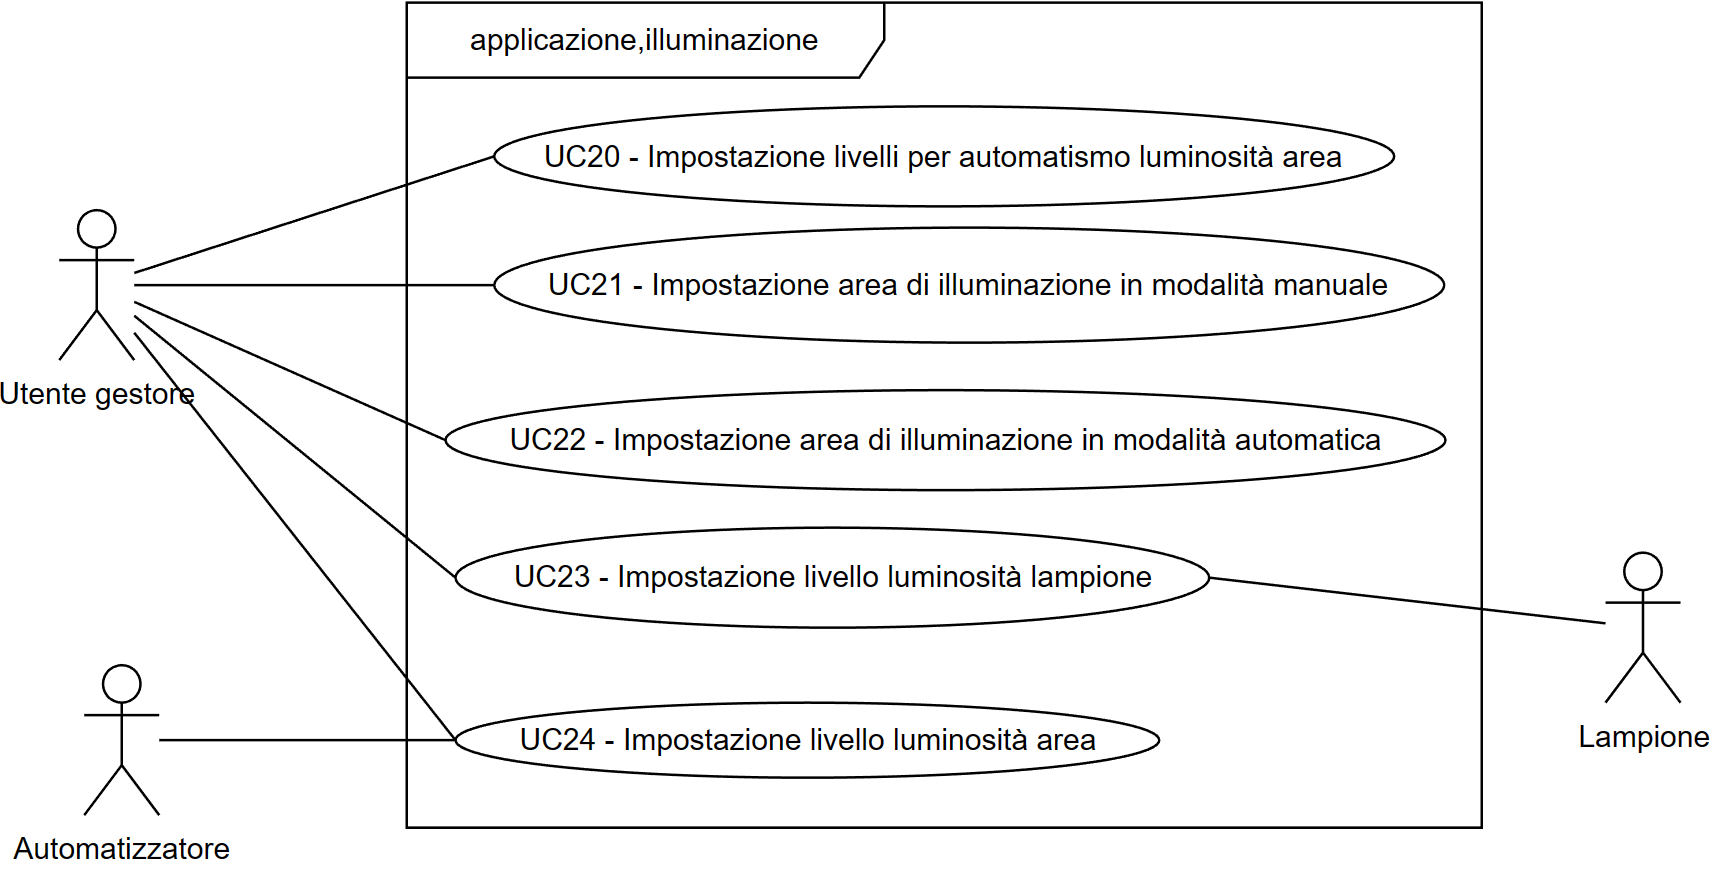
\includegraphics[width=\textwidth]{contenuti/img/casi_uso_grafici-applicazione,illuminazione.png}
    \caption{Parte dell'applicazione relativa alla gestione dell'illuminazione}
    \label{fig:illuminazione}
\end{figure}

\subsection{I casi d'uso descritti}

\begin{itemize}
    \item \hyperref[uc:20]{UC20 - Impostare livelli per automatismo luminosità area}
    \item \hyperref[uc:21]{UC21 - Impostazione area di illuminazione in modalità manuale}
    \item \hyperref[uc:22]{UC22 - Impostare area di illuminazione in modalità automatica}
    \item \hyperref[uc:23]{UC23 - Impostazione livello luminosità lampione}
    \item \hyperref[uc:24]{UC24 - Impostare livello luminosità area}
\end{itemize}
